\documentclass[letterpaper,12pt]{article}
\usepackage[margin=.65in,top=.72in,bottom=.62in,headheight=16pt,headsep=15pt,footskip=19pt]{geometry}
\usepackage[T1]{fontenc}
\usepackage{lmodern,tikz,fancyhdr}\pdfmapfile{+lm.map}
\usetikzlibrary{arrows.meta,shapes.geometric}
\pagestyle{fancy}\fancyhf{}\renewcommand{\headrulewidth}{0pt}\renewcommand{\footrulewidth}{0pt}
\setlength{\parindent}{0pt}\setlength{\parskip}{0pt}
\fancyhead[L]{\small Week 45 / The visible side / Grades 4--5}
\fancyfoot[L]{\footnotesize Bellingham Math Circle / Week 45 / W45-grades-4-5-v2}\fancyfoot[R]{\footnotesize\thepage}
\begin{document}
\noindent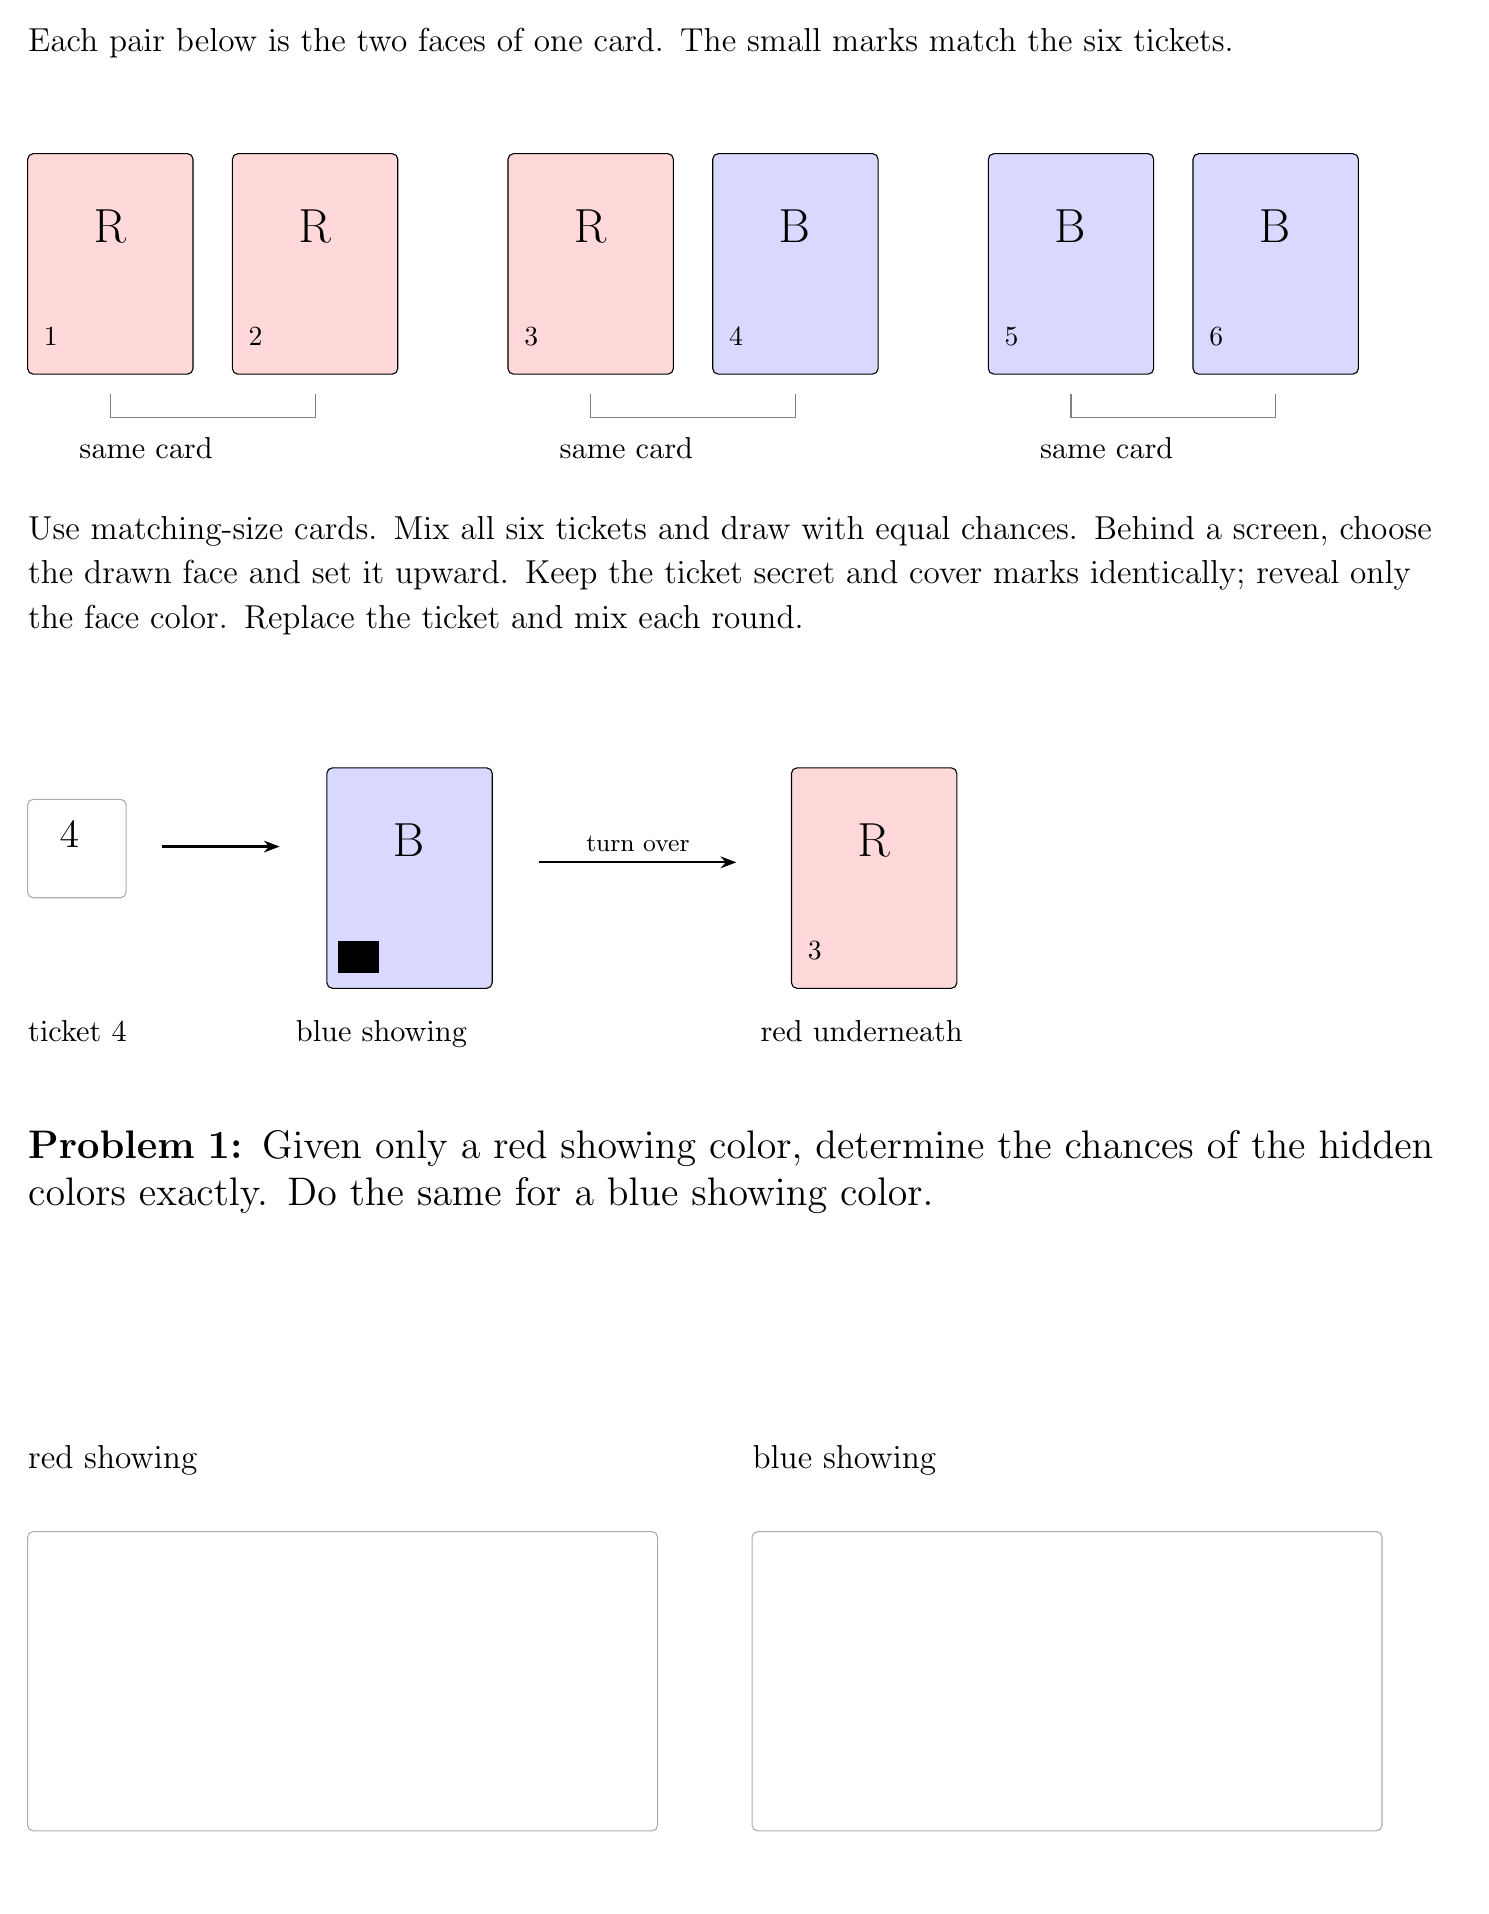
\begin{tikzpicture}[x=1cm,y=1cm]\path[use as bounding box] (0,0) rectangle (18.2,-23.6);
\node[anchor=north west,text width=18cm,inner sep=0pt,font=\fontsize{13}{16}\selectfont] at (0,0) {Each pair below is the two faces of one card. The small marks match the six tickets.};
\draw[fill=red!15,rounded corners=2pt] (0.0,-1.6) rectangle (2.1,-4.4);
\node[anchor=north west,text width=0.6cm,inner sep=0pt,font=\fontsize{17}{20}\selectfont] at (0.8300000000000001,-2.3) {R};
\node[anchor=north west,text width=0.7cm,inner sep=0pt,font=\fontsize{10}{13}\selectfont] at (0.2,-3.8000000000000003) {1};
\draw[fill=red!15,rounded corners=2pt] (2.6,-1.6) rectangle (4.7,-4.4);
\node[anchor=north west,text width=0.6cm,inner sep=0pt,font=\fontsize{17}{20}\selectfont] at (3.43,-2.3) {R};
\node[anchor=north west,text width=0.7cm,inner sep=0pt,font=\fontsize{10}{13}\selectfont] at (2.8000000000000003,-3.8000000000000003) {2};
\draw[gray] (1.05,-4.65) -- (1.05,-4.95) -- (3.65,-4.95) -- (3.65,-4.65);
\node[anchor=north west,text width=4cm,inner sep=0pt,font=\fontsize{11}{14}\selectfont] at (0.65,-5.2) {same card};
\draw[fill=red!15,rounded corners=2pt] (6.1,-1.6) rectangle (8.2,-4.4);
\node[anchor=north west,text width=0.6cm,inner sep=0pt,font=\fontsize{17}{20}\selectfont] at (6.93,-2.3) {R};
\node[anchor=north west,text width=0.7cm,inner sep=0pt,font=\fontsize{10}{13}\selectfont] at (6.3,-3.8000000000000003) {3};
\draw[fill=blue!15,rounded corners=2pt] (8.7,-1.6) rectangle (10.799999999999999,-4.4);
\node[anchor=north west,text width=0.6cm,inner sep=0pt,font=\fontsize{17}{20}\selectfont] at (9.53,-2.3) {B};
\node[anchor=north west,text width=0.7cm,inner sep=0pt,font=\fontsize{10}{13}\selectfont] at (8.899999999999999,-3.8000000000000003) {4};
\draw[gray] (7.1499999999999995,-4.65) -- (7.1499999999999995,-4.95) -- (9.75,-4.95) -- (9.75,-4.65);
\node[anchor=north west,text width=4cm,inner sep=0pt,font=\fontsize{11}{14}\selectfont] at (6.75,-5.2) {same card};
\draw[fill=blue!15,rounded corners=2pt] (12.2,-1.6) rectangle (14.299999999999999,-4.4);
\node[anchor=north west,text width=0.6cm,inner sep=0pt,font=\fontsize{17}{20}\selectfont] at (13.03,-2.3) {B};
\node[anchor=north west,text width=0.7cm,inner sep=0pt,font=\fontsize{10}{13}\selectfont] at (12.399999999999999,-3.8000000000000003) {5};
\draw[fill=blue!15,rounded corners=2pt] (14.799999999999999,-1.6) rectangle (16.9,-4.4);
\node[anchor=north west,text width=0.6cm,inner sep=0pt,font=\fontsize{17}{20}\selectfont] at (15.629999999999999,-2.3) {B};
\node[anchor=north west,text width=0.7cm,inner sep=0pt,font=\fontsize{10}{13}\selectfont] at (14.999999999999998,-3.8000000000000003) {6};
\draw[gray] (13.25,-4.65) -- (13.25,-4.95) -- (15.85,-4.95) -- (15.85,-4.65);
\node[anchor=north west,text width=4cm,inner sep=0pt,font=\fontsize{11}{14}\selectfont] at (12.85,-5.2) {same card};
\node[anchor=north west,text width=18cm,inner sep=0pt,font=\fontsize{13}{16}\selectfont] at (0,-6.2) {Use matching-size cards. Mix all six tickets and draw with equal chances. Behind a screen, choose the drawn face and set it upward. Keep the ticket secret and cover marks identically; reveal only the face color. Replace the ticket and mix each round.};
\draw[gray!65,rounded corners=2pt] (0,-9.8) rectangle (1.25,-11.05);
\node[anchor=north west,text width=0.5cm,inner sep=0pt,font=\fontsize{14}{17}\selectfont] at (0.4,-10.08) {4};
\draw[-{Stealth[length=2mm]},line width=.8pt] (1.7,-10.4) -- (3.2,-10.4) node[midway,above,font=\small] {};
\draw[fill=blue!15,rounded corners=2pt] (3.8,-9.4) rectangle (5.9,-12.2);
\node[anchor=north west,text width=0.6cm,inner sep=0pt,font=\fontsize{17}{20}\selectfont] at (4.63,-10.1) {B};
\draw[fill=black] (3.9499999999999997,-12.0) rectangle (4.45,-11.6);
\draw[-{Stealth[length=2mm]},line width=.8pt] (6.5,-10.6) -- (9,-10.6) node[midway,above,font=\small] {turn over};
\draw[fill=red!15,rounded corners=2pt] (9.7,-9.4) rectangle (11.799999999999999,-12.2);
\node[anchor=north west,text width=0.6cm,inner sep=0pt,font=\fontsize{17}{20}\selectfont] at (10.53,-10.1) {R};
\node[anchor=north west,text width=0.7cm,inner sep=0pt,font=\fontsize{10}{13}\selectfont] at (9.899999999999999,-11.6) {3};
\node[anchor=north west,text width=3cm,inner sep=0pt,font=\fontsize{11}{14}\selectfont] at (0,-12.6) {ticket 4};
\node[anchor=north west,text width=5cm,inner sep=0pt,font=\fontsize{11}{14}\selectfont] at (3.4,-12.6) {blue showing};
\node[anchor=north west,text width=7cm,inner sep=0pt,font=\fontsize{11}{14}\selectfont] at (9.3,-12.6) {red underneath};
\node[anchor=north west,text width=18cm,inner sep=0pt,font=\fontsize{14}{17}\selectfont] at (0,-14) {\textbf{Problem 1:} Given only a red showing color, determine the chances of the hidden colors exactly. Do the same for a blue showing color.};
\node[anchor=north west,text width=8cm,inner sep=0pt,font=\fontsize{13}{16}\selectfont] at (0.0,-18) {red showing};
\draw[gray!65,rounded corners=2pt] (0.0,-19.1) rectangle (8.0,-22.900000000000002);
\node[anchor=north west,text width=8cm,inner sep=0pt,font=\fontsize{13}{16}\selectfont] at (9.2,-18) {blue showing};
\draw[gray!65,rounded corners=2pt] (9.2,-19.1) rectangle (17.2,-22.900000000000002);
\end{tikzpicture}
\newpage
\noindent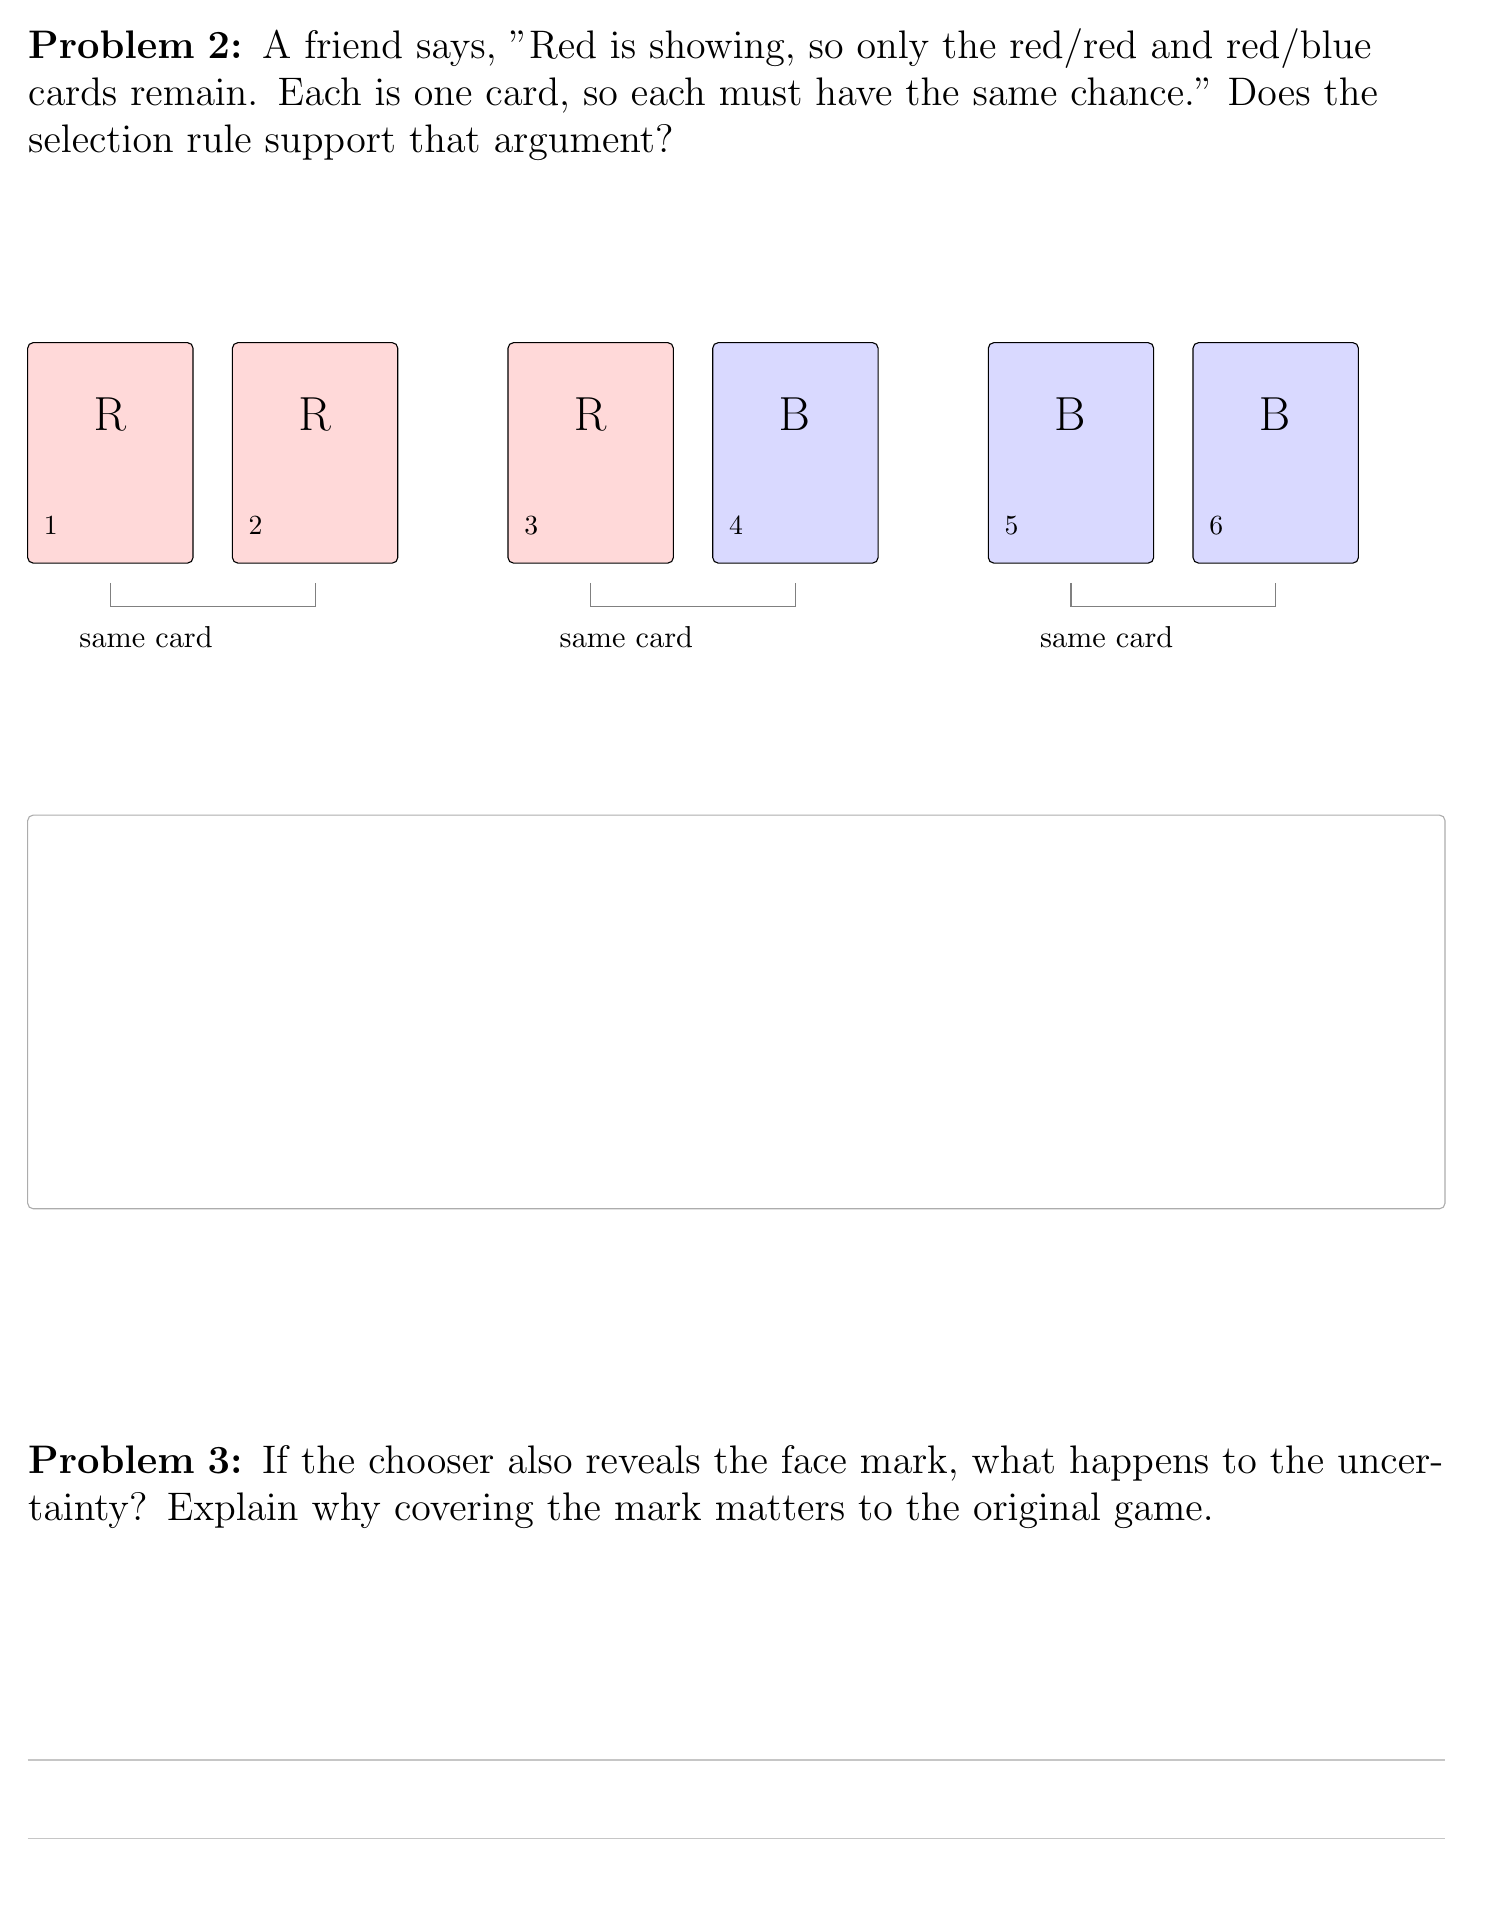
\begin{tikzpicture}[x=1cm,y=1cm]\path[use as bounding box] (0,0) rectangle (18.2,-23.6);
\node[anchor=north west,text width=18cm,inner sep=0pt,font=\fontsize{14}{17}\selectfont] at (0,0) {\textbf{Problem 2:} A friend says, "Red is showing, so only the red/red and red/blue cards remain. Each is one card, so each must have the same chance." Does the selection rule support that argument?};
\draw[fill=red!15,rounded corners=2pt] (0.0,-4) rectangle (2.1,-6.8);
\node[anchor=north west,text width=0.6cm,inner sep=0pt,font=\fontsize{17}{20}\selectfont] at (0.8300000000000001,-4.7) {R};
\node[anchor=north west,text width=0.7cm,inner sep=0pt,font=\fontsize{10}{13}\selectfont] at (0.2,-6.2) {1};
\draw[fill=red!15,rounded corners=2pt] (2.6,-4) rectangle (4.7,-6.8);
\node[anchor=north west,text width=0.6cm,inner sep=0pt,font=\fontsize{17}{20}\selectfont] at (3.43,-4.7) {R};
\node[anchor=north west,text width=0.7cm,inner sep=0pt,font=\fontsize{10}{13}\selectfont] at (2.8000000000000003,-6.2) {2};
\draw[gray] (1.05,-7.05) -- (1.05,-7.35) -- (3.65,-7.35) -- (3.65,-7.05);
\node[anchor=north west,text width=4cm,inner sep=0pt,font=\fontsize{11}{14}\selectfont] at (0.65,-7.6) {same card};
\draw[fill=red!15,rounded corners=2pt] (6.1,-4) rectangle (8.2,-6.8);
\node[anchor=north west,text width=0.6cm,inner sep=0pt,font=\fontsize{17}{20}\selectfont] at (6.93,-4.7) {R};
\node[anchor=north west,text width=0.7cm,inner sep=0pt,font=\fontsize{10}{13}\selectfont] at (6.3,-6.2) {3};
\draw[fill=blue!15,rounded corners=2pt] (8.7,-4) rectangle (10.799999999999999,-6.8);
\node[anchor=north west,text width=0.6cm,inner sep=0pt,font=\fontsize{17}{20}\selectfont] at (9.53,-4.7) {B};
\node[anchor=north west,text width=0.7cm,inner sep=0pt,font=\fontsize{10}{13}\selectfont] at (8.899999999999999,-6.2) {4};
\draw[gray] (7.1499999999999995,-7.05) -- (7.1499999999999995,-7.35) -- (9.75,-7.35) -- (9.75,-7.05);
\node[anchor=north west,text width=4cm,inner sep=0pt,font=\fontsize{11}{14}\selectfont] at (6.75,-7.6) {same card};
\draw[fill=blue!15,rounded corners=2pt] (12.2,-4) rectangle (14.299999999999999,-6.8);
\node[anchor=north west,text width=0.6cm,inner sep=0pt,font=\fontsize{17}{20}\selectfont] at (13.03,-4.7) {B};
\node[anchor=north west,text width=0.7cm,inner sep=0pt,font=\fontsize{10}{13}\selectfont] at (12.399999999999999,-6.2) {5};
\draw[fill=blue!15,rounded corners=2pt] (14.799999999999999,-4) rectangle (16.9,-6.8);
\node[anchor=north west,text width=0.6cm,inner sep=0pt,font=\fontsize{17}{20}\selectfont] at (15.629999999999999,-4.7) {B};
\node[anchor=north west,text width=0.7cm,inner sep=0pt,font=\fontsize{10}{13}\selectfont] at (14.999999999999998,-6.2) {6};
\draw[gray] (13.25,-7.05) -- (13.25,-7.35) -- (15.85,-7.35) -- (15.85,-7.05);
\node[anchor=north west,text width=4cm,inner sep=0pt,font=\fontsize{11}{14}\selectfont] at (12.85,-7.6) {same card};
\draw[gray!65,rounded corners=2pt] (0,-10) rectangle (18,-15);
\node[anchor=north west,text width=18cm,inner sep=0pt,font=\fontsize{14}{17}\selectfont] at (0,-18) {\textbf{Problem 3:} If the chooser also reveals the face mark, what happens to the uncertainty? Explain why covering the mark matters to the original game.};
\draw[gray!45] (0,-22) -- (18,-22);
\draw[gray!45] (0,-23) -- (18,-23);
\end{tikzpicture}
\newpage
\noindent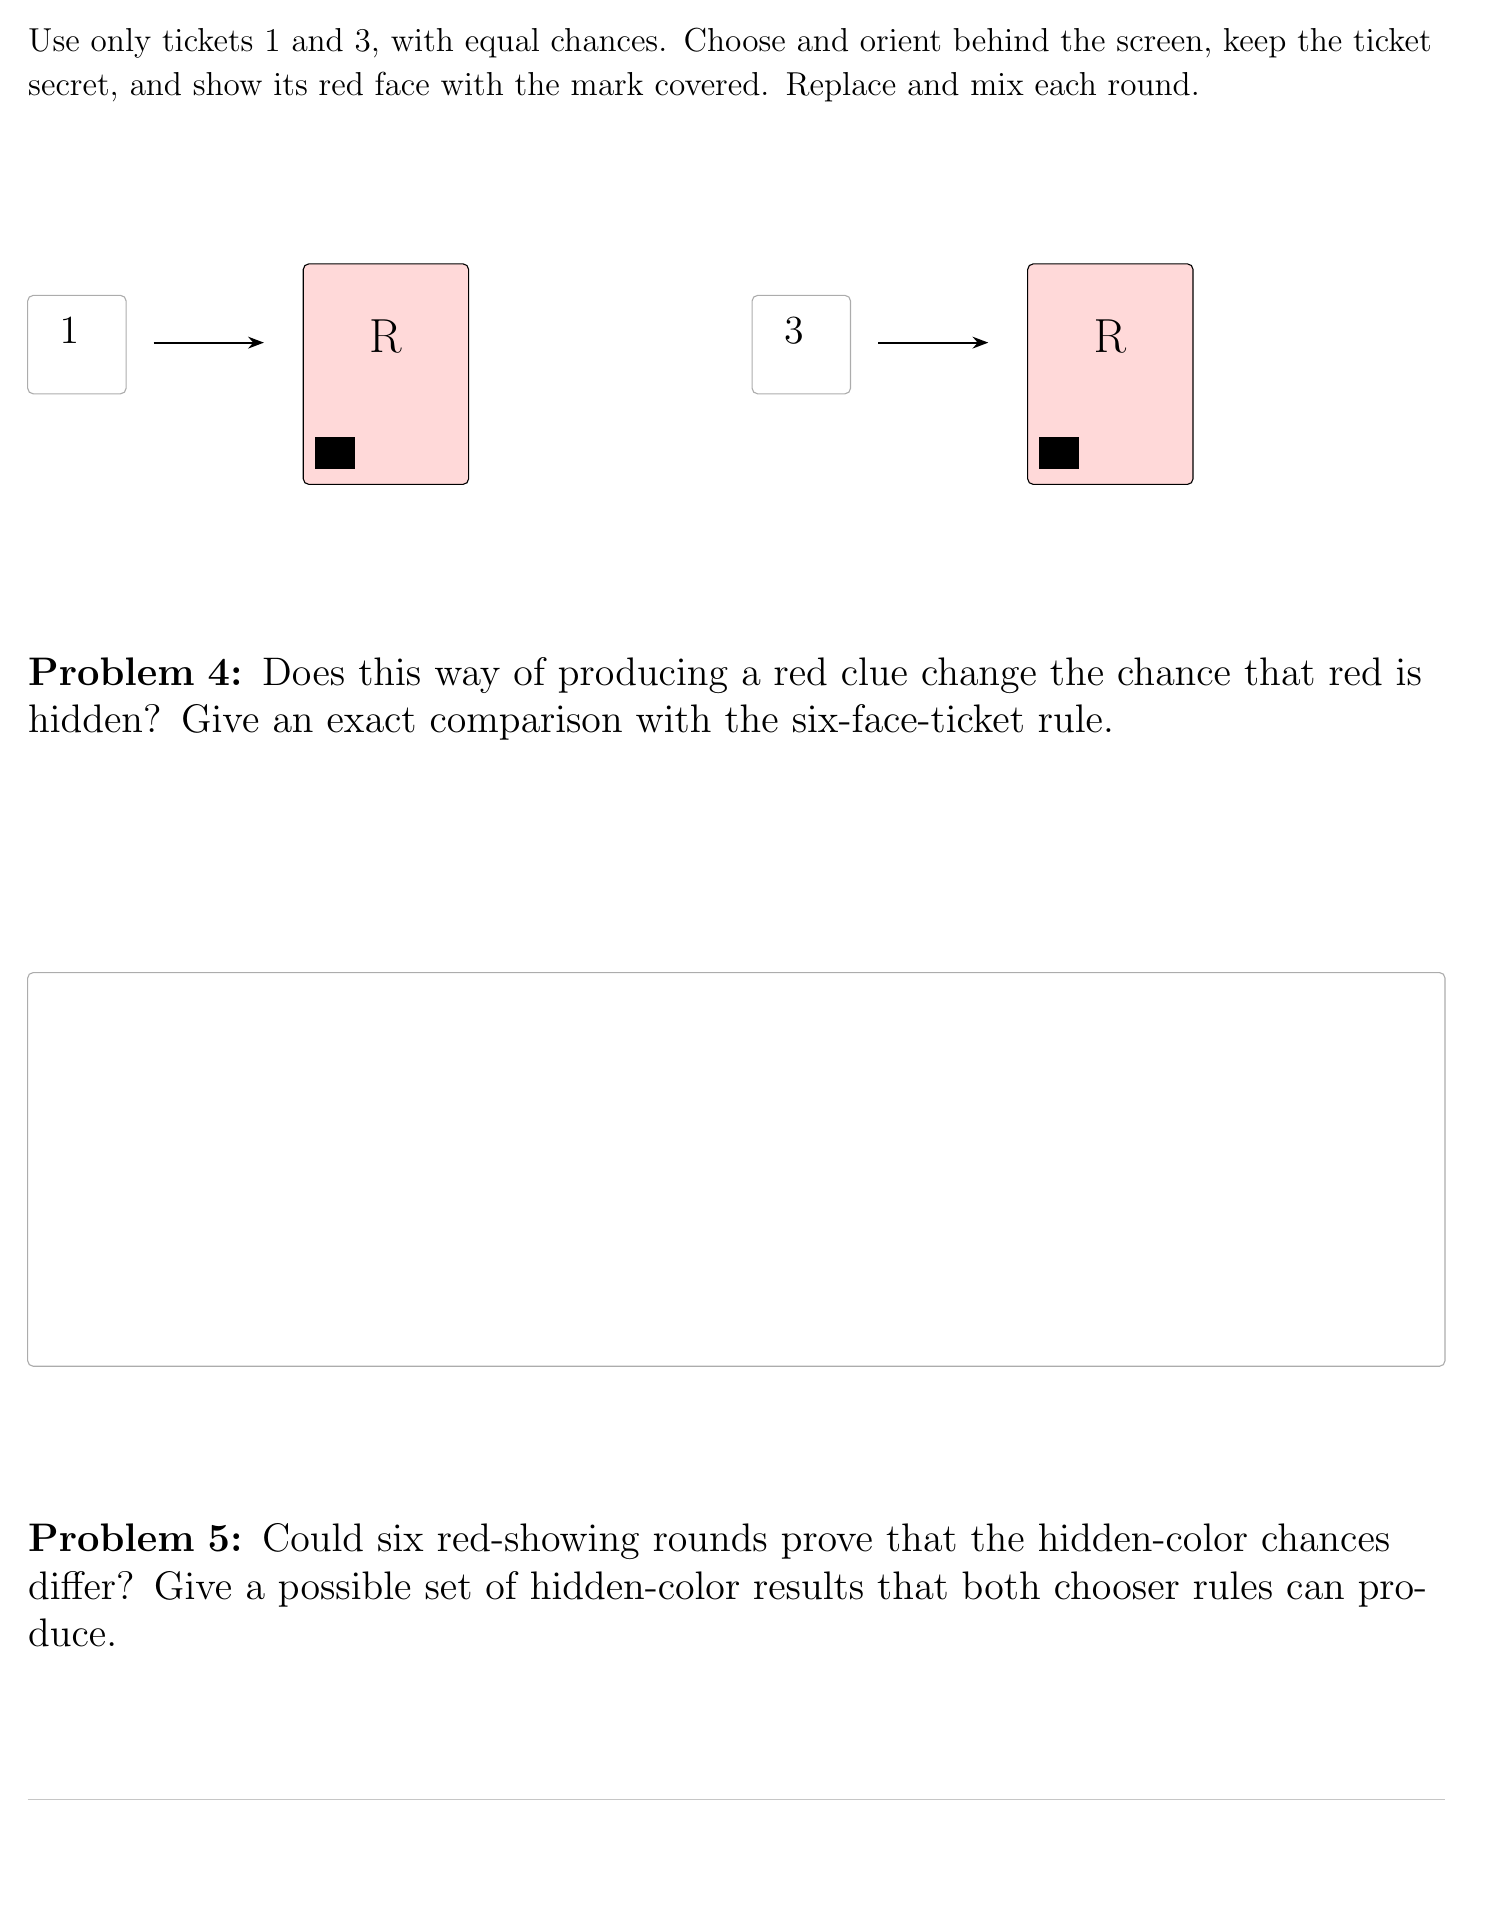
\begin{tikzpicture}[x=1cm,y=1cm]\path[use as bounding box] (0,0) rectangle (18.2,-23.6);
\node[anchor=north west,text width=18cm,inner sep=0pt,font=\fontsize{13}{16}\selectfont] at (0,0) {Use only tickets 1 and 3, with equal chances. Choose and orient behind the screen, keep the ticket secret, and show its red face with the mark covered. Replace and mix each round.};
\draw[gray!65,rounded corners=2pt] (0,-3.4) rectangle (1.25,-4.65);
\node[anchor=north west,text width=0.5cm,inner sep=0pt,font=\fontsize{14}{17}\selectfont] at (0.4,-3.6799999999999997) {1};
\draw[-{Stealth[length=2mm]},line width=.8pt] (1.6,-4) -- (3,-4) node[midway,above,font=\small] {};
\draw[fill=red!15,rounded corners=2pt] (3.5,-3) rectangle (5.6,-5.8);
\node[anchor=north west,text width=0.6cm,inner sep=0pt,font=\fontsize{17}{20}\selectfont] at (4.33,-3.7) {R};
\draw[fill=black] (3.65,-5.6) rectangle (4.15,-5.2);
\draw[gray!65,rounded corners=2pt] (9.2,-3.4) rectangle (10.45,-4.65);
\node[anchor=north west,text width=0.5cm,inner sep=0pt,font=\fontsize{14}{17}\selectfont] at (9.6,-3.6799999999999997) {3};
\draw[-{Stealth[length=2mm]},line width=.8pt] (10.799999999999999,-4) -- (12.2,-4) node[midway,above,font=\small] {};
\draw[fill=red!15,rounded corners=2pt] (12.7,-3) rectangle (14.799999999999999,-5.8);
\node[anchor=north west,text width=0.6cm,inner sep=0pt,font=\fontsize{17}{20}\selectfont] at (13.53,-3.7) {R};
\draw[fill=black] (12.85,-5.6) rectangle (13.35,-5.2);
\node[anchor=north west,text width=18cm,inner sep=0pt,font=\fontsize{14}{17}\selectfont] at (0,-8) {\textbf{Problem 4:} Does this way of producing a red clue change the chance that red is hidden? Give an exact comparison with the six-face-ticket rule.};
\draw[gray!65,rounded corners=2pt] (0,-12) rectangle (18,-17);
\node[anchor=north west,text width=18cm,inner sep=0pt,font=\fontsize{14}{17}\selectfont] at (0,-19) {\textbf{Problem 5:} Could six red-showing rounds prove that the hidden-color chances differ? Give a possible set of hidden-color results that both chooser rules can produce.};
\draw[gray!45] (0,-22.5) -- (18,-22.5);
\end{tikzpicture}
\newpage
\noindent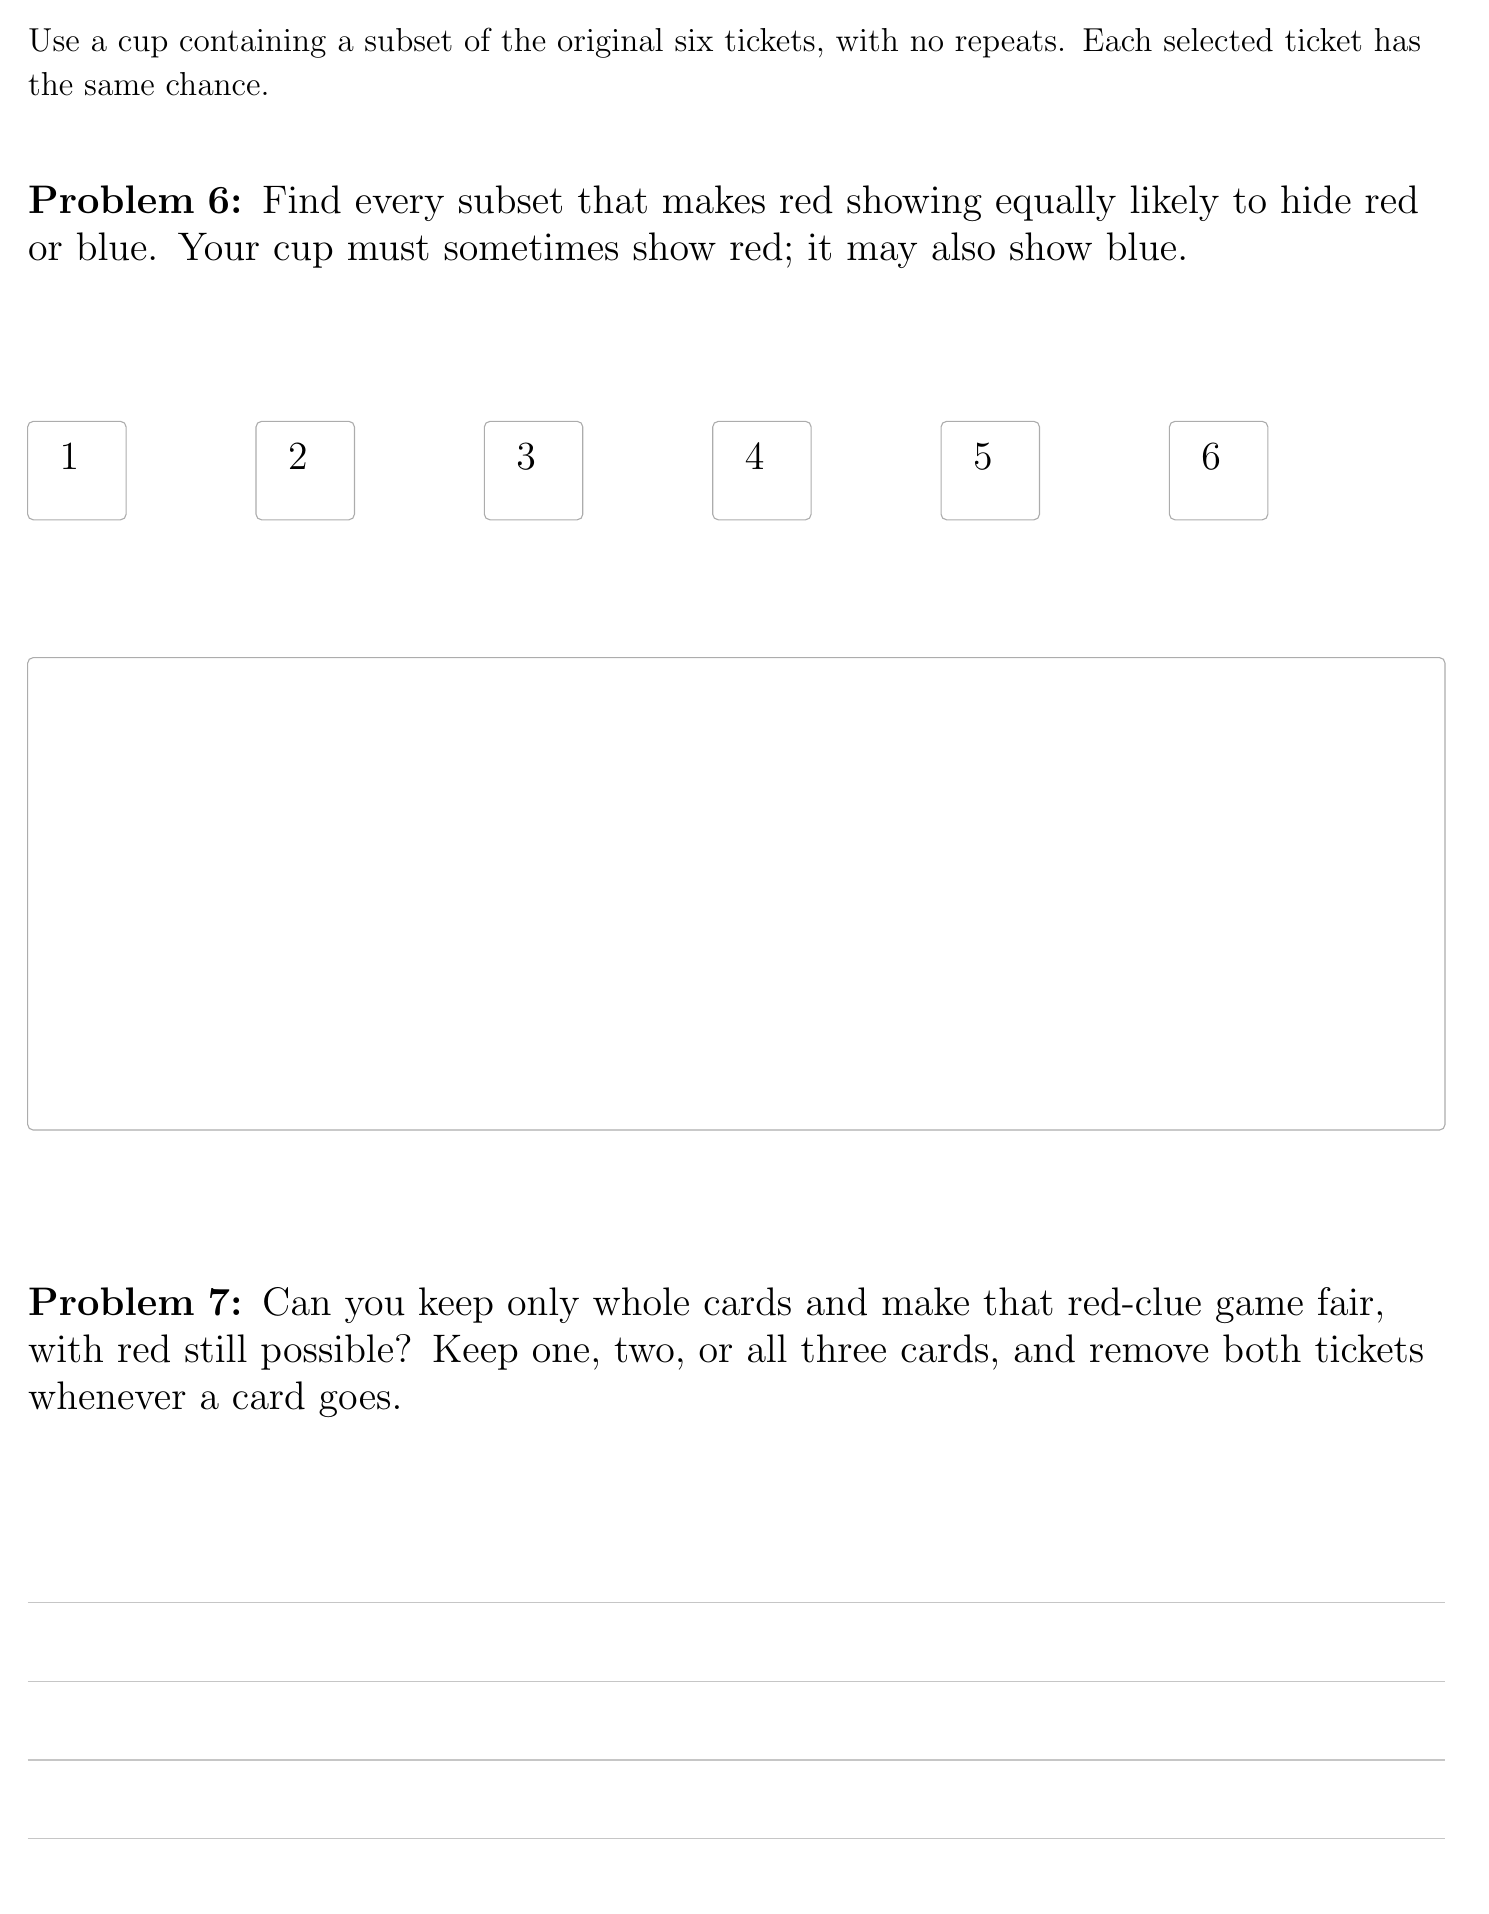
\begin{tikzpicture}[x=1cm,y=1cm]\path[use as bounding box] (0,0) rectangle (18.2,-23.6);
\node[anchor=north west,text width=18cm,inner sep=0pt,font=\fontsize{13}{16}\selectfont] at (0,0) {Use a cup containing a subset of the original six tickets, with no repeats. Each selected ticket has the same chance.};
\node[anchor=north west,text width=18cm,inner sep=0pt,font=\fontsize{14}{17}\selectfont] at (0,-2) {\textbf{Problem 6:} Find every subset that makes red showing equally likely to hide red or blue. Your cup must sometimes show red; it may also show blue.};
\draw[gray!65,rounded corners=2pt] (0.0,-5) rectangle (1.25,-6.25);
\node[anchor=north west,text width=0.5cm,inner sep=0pt,font=\fontsize{14}{17}\selectfont] at (0.4,-5.28) {1};
\draw[gray!65,rounded corners=2pt] (2.9,-5) rectangle (4.15,-6.25);
\node[anchor=north west,text width=0.5cm,inner sep=0pt,font=\fontsize{14}{17}\selectfont] at (3.3,-5.28) {2};
\draw[gray!65,rounded corners=2pt] (5.8,-5) rectangle (7.05,-6.25);
\node[anchor=north west,text width=0.5cm,inner sep=0pt,font=\fontsize{14}{17}\selectfont] at (6.2,-5.28) {3};
\draw[gray!65,rounded corners=2pt] (8.7,-5) rectangle (9.95,-6.25);
\node[anchor=north west,text width=0.5cm,inner sep=0pt,font=\fontsize{14}{17}\selectfont] at (9.1,-5.28) {4};
\draw[gray!65,rounded corners=2pt] (11.6,-5) rectangle (12.85,-6.25);
\node[anchor=north west,text width=0.5cm,inner sep=0pt,font=\fontsize{14}{17}\selectfont] at (12.0,-5.28) {5};
\draw[gray!65,rounded corners=2pt] (14.5,-5) rectangle (15.75,-6.25);
\node[anchor=north west,text width=0.5cm,inner sep=0pt,font=\fontsize{14}{17}\selectfont] at (14.9,-5.28) {6};
\draw[gray!65,rounded corners=2pt] (0,-8) rectangle (18,-14);
\node[anchor=north west,text width=18cm,inner sep=0pt,font=\fontsize{14}{17}\selectfont] at (0,-16) {\textbf{Problem 7:} Can you keep only whole cards and make that red-clue game fair, with red still possible? Keep one, two, or all three cards, and remove both tickets whenever a card goes.};
\draw[gray!45] (0,-20) -- (18,-20);
\draw[gray!45] (0,-21) -- (18,-21);
\draw[gray!45] (0,-22) -- (18,-22);
\draw[gray!45] (0,-23) -- (18,-23);
\end{tikzpicture}
\end{document}
